\documentclass{IEEEtran}
\usepackage{graphicx}
\usepackage{fancyhdr}
\usepackage{listings}

\graphicspath{ {images/} }
\pagestyle{fancy}
\fancyhf{}
\rhead{Segundo Proyecto Programado}
\rfoot{P\'agina \thepage}

\begin{document}
\begin{titlepage}
  \centering
  {\scshape\LARGE Instituto Tecnol\'ogico de Costa Rica \par}
  \vspace{1cm}
  {\scshape\Large Segundo proyecto programado\par}
  \vspace{1.5cm}
  {\Large\itshape Ariel Herrera\par}
  {\Large\itshape Sa\'ul Zamora\par}
  \vfill
  profesor\par
  M. Sc. Sa\'ul Calder\'on Ram\'irez \textsc{}

  \vfill

% Bottom of the page
  {\large \today\par}
\end{titlepage}

\section{Introducci\'on}
En la actualidad, los sistemas de almacenamiento y comunicaci\'on digitales requieren de m\'etodos optimizados para el uso de recursos (energ\'eticos, temporales, de estacio, etc). Para satisfacer tal necesidad de manera efectiva, muchas disciplinas han formulado m\'utiples algoritmis para comprimir y descomprimir la informaci\'on. La compresi\'on de datos consiste en aplicar alg\'un m\'etodo que permita reducir el tama\~no original de la informaci\'on. Los algoritmos de compresi\'on sin p\'erdida son capaces de aplicar una serie de pasos para construir la informaci\'on comprimida, para luego, cuando la informaci\'on original necesite ser accesada, se descomprime y recupera la informaci\'on original complemtamente id\'entica. Los algoritmos de compresi\'on con p\'erdida en cambio, al implementar la descompresi\'on de la informaci\'on, no lo gran recuperar el 100\% de los datos originales. El algoritmo de Huffman implementado en este proyecto fue propuesto por David A. Huffman en 1952 enfocado en la compresi\'on sin p\'erdida de datos.

\section{An\'alisis del problema}
La t\'ecnica de Huffman trabaja al crear un \'arbol binario de nodos, los cuales pueden ser hojas o nodos internos. Al principio, todos empiezan como hojas, las cuales contienen un s\'imbolo, el peso (\emph{frecuencia}) es opcional, y un enlace al nodo padre, lo cual facilita leer el c\'odigo comenzando de las hojas. Los nodos internos contienen el peso del s\'imbolo, dos enlaces a nodos hijos y un enlace opcional a un nodo padre.

Como una convenci\'on, el bit \emph{0} representa el siguiente hijo izquierdo y el bit \emph{1} el siguiente hijo derecho. Un \'arbol terminado puede crecer hasta tener ($n$) hojas y ($n - 1$) nodos internos. Un \'arbol de Huffman que omite los s\'imbolos que no se usan, produce el c\'odigo con el largo \'optimo.

El proceso inicia con las hojas conteniendolos s\'imbolos a representar, luego un nuevo nodo es creado con los nodos con menor probalilidad como hijos, tal que la probabilidad de dicho nodo es igual a la suma de las probabilidades de sus hijos. Con los nodos anteriores mezclados en uno (ya no son considerados), y considerando al nuevo nodo, el proceso se repite hasta que solo quede un nodo: el \'arbol de Huffman.
\section{Dise\~no de la soluci\'on}
\subsection{El algoritmo de Huffman}
El algoritmo de Huffman fue dise\~nado para comprimir se\~nales digitales. Dichas se\~nales est\'an compuestas por un conjunto finito de s\'imbolos, donde cada uno est\'a definido por una cadena de bits.

El algoritmo de Huffman busca crear para cada s\'imbolo, una cadena de bits o c\'odigo de Huffman, que al reemplazarse por el \emph{token} correspondiente, reduzca el tama\~no total del texto. Para construir el diccionario, el algoritmo analiza todo el texto, para construir un diccionario de frecuencias de aparici\'on, el cual defina una entrada por \emph{token}, donde dicho \emph{token} es la llave y el valor de entrada es definido por la cantidad de veces que el \emph{token} aparece en el texto.

El algoritmo busca generar el c\'odigo m\'as corto para el s\'imbolo m\'as recurrente. Para ello es necesario asegurarse que la codificaci\'on de todos los tokens no sea ambigua, es decir, que sea posible reconstruir el texto original a partir de la se\~nal codificada. Para ello, se utiliza el \'arbol binario como estructura de datos.

\subsection{El \'arbol binario}
El \'arbol binario es una estructura de datos que est\'a compuesta por un conjunto de nodos. Un nodo se entiende como una estructura que puede contener cualquier tipo de dato en su interior. Los datos dentro del nodo forman la \emph{etiqueta} del mismo. Un nodo puede estar enlazado como m\'aximo, a dos nodos (de ah\'i el nombre, \emph{\'arbol binario}), los cuales est\'an en un nivel jer\'arquico inferior.

Un nodo tiene como propiedades su etiqueta, un hijo izquierdo y un hijo derecho. Tales propiedades definen sus operaciones b\'asicas: \emph{crearNodo(nodo)}, que recibe como m\'inimo la etiqueta como argumento y las inserciones de los nodos izquierdos y derechos \emph{insertarHijoIzquierdo(nodo)} e \emph{insertarHijoDerecho(nodo)} respectivamente.

\subsubsection{Estructura b\'asica de un \'arbol binario}
\begin{itemize}
  \item Ra\'iz: es el \'unico nodo que no desciende de ning\'un otro. Es el nodo jer\'arquicamente superior.
  \item Nodos hoja: se definen como aquellos nodos que no tienen descendientes.
\end{itemize}

\subsection{Huffman y el \'arbol binario}
El algoritmo consiste en construir el \'arbol binario \emph{de abajo hacia arriba} para definir el c\'odigo de cada token. Al terminar de construir el \'arbol, existir\'a un nodo por cada token, y que tambi\'en contendr\'a la cantidad total de repeticiones de todos los nodos hijos, en cada nodo.

Los pasos para construir el \'arbol es la siguiente:
\begin{enumerate}
  \item Crear un nodo por cada token, incluyendo en su etiqueta el n\'umero de repeticiones en el texto. Agregar todos los nodos a una lista.
  \item Tomar y remover los dos nodos de menor frecuencia de la lista y unirlos en un nuevo nodo, el cual tendr\'a los dos nodos con menor frecuencia como hijos. Este nuevo nodo tendr\'a como etiqueta un token nulo, y como cantidad de apariciones, la suma de la cantidad de apariciones de los nodos hijos. El nuevo nodo se inserta en la lista de nodos.
  \item Repetir el paso 2 hasta que exista un solo nodo en la lista. Cuando exista un \'unico nodo en la lista de nodos, el mismo se toma como ra\'iz del \'arbol de Huffman.
\end{enumerate}

El \'arbol de Huffman es utilizado para construir el c\'odigo de Huffman para cada token. Dada la naturaleza del algoritmo, los tokens con mayor cantidad de apariciones en el texto son incluidos de \'ultimo en el \'arbol, por lo que estar\'an m\'as cerca de la ra\'iz del \'arbol binario.

\subsection{Pseudoc\'odigo}

\lstinputlisting[language=Prolog, basicstyle=\tiny]{Pseudo.txt}

\section{Pruebas}

\begin{figure}[!ht]
  \caption{Texto de Prueba 1}
  \centering
    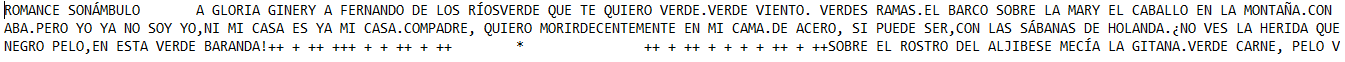
\includegraphics[width=0.4\textwidth]{Prueba_1.png}
\end{figure}

\begin{figure}[!ht]
  \caption{Diccionario 1}
  \centering
    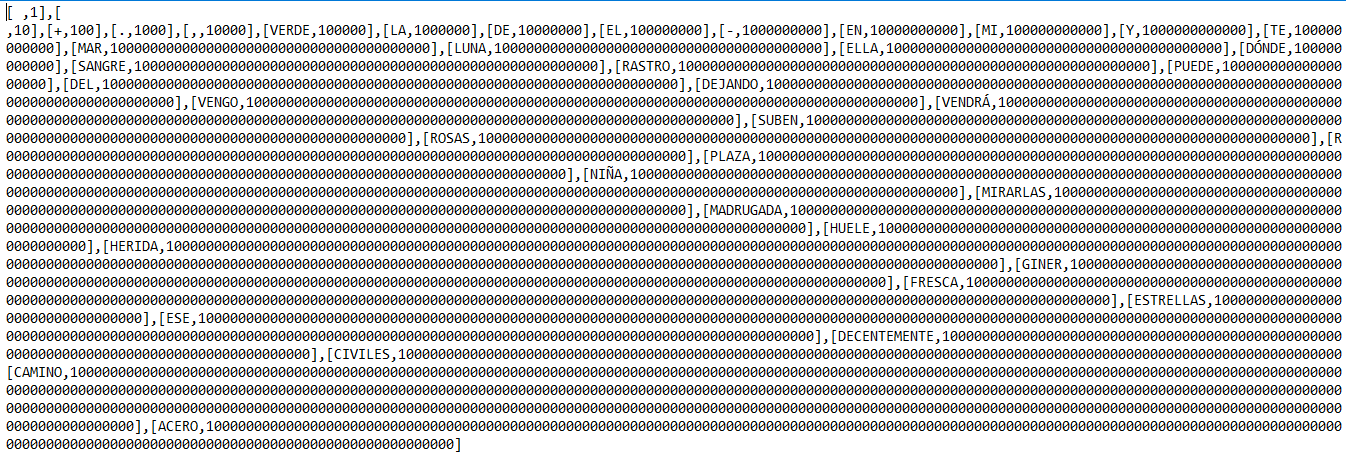
\includegraphics[width=0.4\textwidth]{Prueba_2.png}
\end{figure}

\begin{figure}[!ht]
  \caption{Texto comprimido 1}
  \centering
    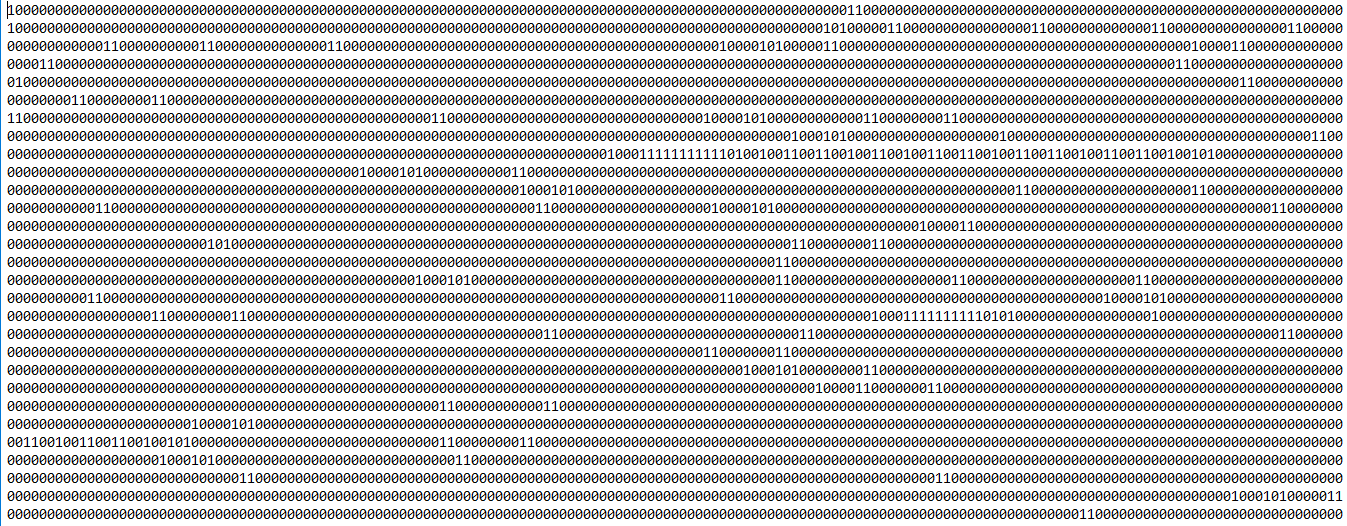
\includegraphics[width=0.4\textwidth]{Prueba_3.png}
\end{figure}

\begin{figure}[!ht]
  \caption{Diccionario 2}
  \centering
    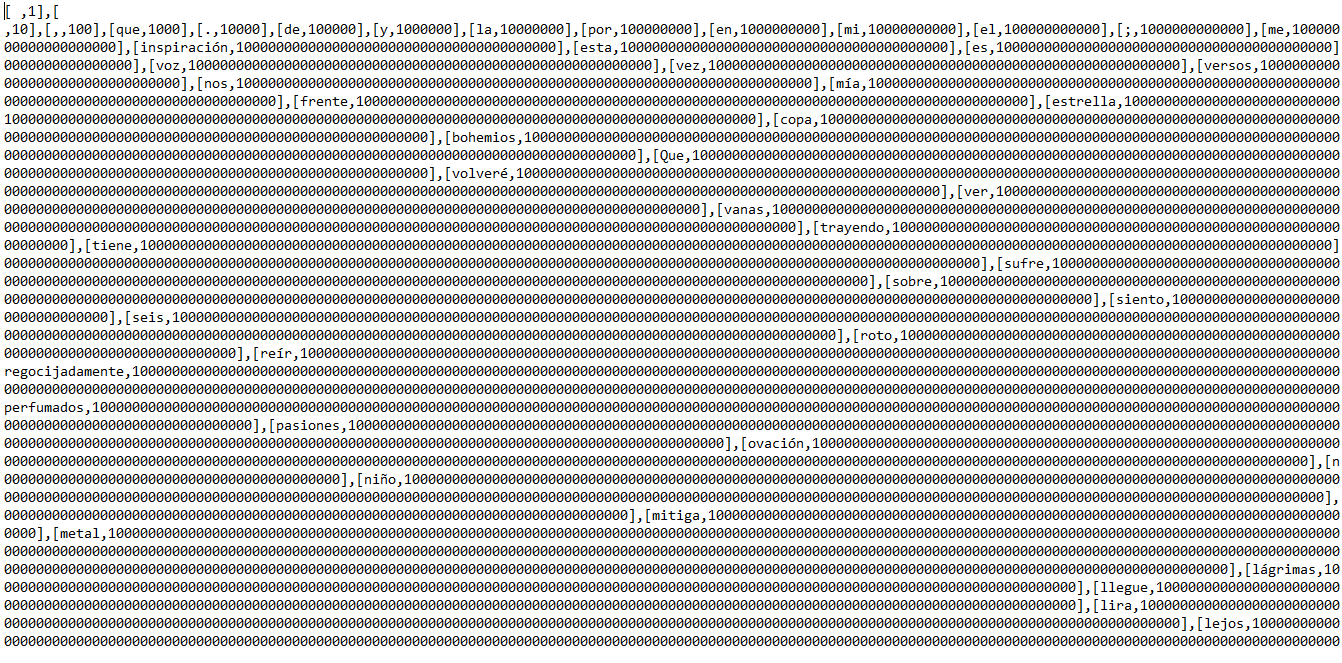
\includegraphics[width=0.4\textwidth]{Prueba_4.png}
\end{figure}

\begin{figure}[!ht]
  \caption{Texto comprimido 2}
  \centering
    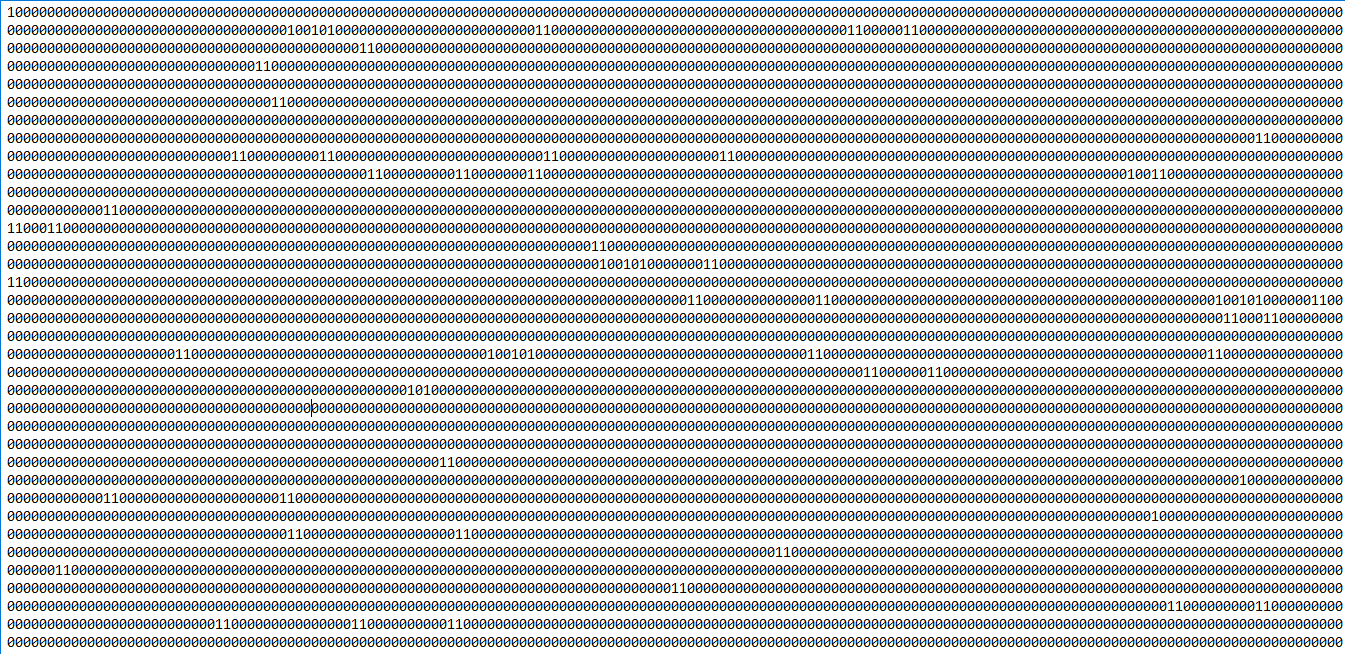
\includegraphics[width=0.4\textwidth]{Prueba_5.png}
\end{figure}

\begin{figure}[!ht]
  \caption{Texto de prueba 2}
  \centering
    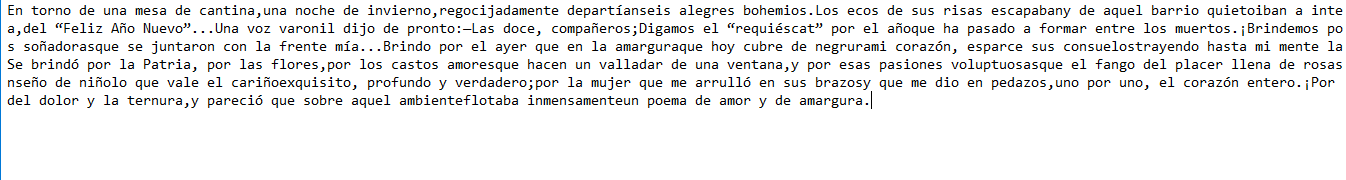
\includegraphics[width=0.4\textwidth]{Prueba_6.png}
\end{figure}

\section{Referencias}

\begin{thebibliography}{99}

\bibitem{huffman} Mamta  Sharma.   Compression  using  Huffman  coding. \emph{IJCSNS International Journal of Computer Science andNetwork Security}, 10(5):133–141, 2010.
\end{thebibliography}
\end{document}